\documentclass{article}
\usepackage{ctex}
\usepackage{bm}
\usepackage{enumitem}
\usepackage{amsmath,amsthm,amsfonts,amssymb}

\def\P{\textbf{P}}
\def\E{\mathbb{E}}
\usepackage{mathtools}
\DeclarePairedDelimiter\ceil{\lceil}{\rceil}
\DeclarePairedDelimiter\abs{\lvert}{\rvert}
\def\X{\mathcal{X}}
\def\Y{\mathcal{Y}}
\usepackage{tikz}
\newtheorem{definition}{定义}
\newtheorem{theorem}{定理}
\author{赵丰}
\title{率失真理论}
\begin{document}
\maketitle

$ X \to \hat{X} $, 通常为多对一的映射。假设用 $J$ bits 描述 $X$, 即 $\hat{X}$ 有 $J$ 个取值, 这些取值称为
再生点或码字。
设 $ X \sim N(0, \sigma^2) $, 失真度量为平方误差, 即寻找 $ \hat{X} $ 使得 $ \E[X - \hat{X} ]^2 $ 最小。
若用 $0$ 比特量化, 取 $ \hat{X} = 0 $ 时平方误差最小。
若用 $1$ 比特量化, 取 $ \hat{X} = \begin{cases} \widehat{X}(0) & x \geq 0 \\ - \widehat{X}(0) & x < 0 \end{cases} $
其中 $ \widehat{X}(0) = 2\int_0^{+\infty} xf(x)dx = \sqrt{2 \over \pi}\sigma $
\begin{definition}
设 $ X^n = (X_1, X_2, \dots, X_n) $, $\widehat{X}^n $ 为 $X^n $ 的表示,$\widehat{X}^n \in \widehat{\mathcal{X}}^n, X^n \in \mathcal{X}^n $。
一个 $(2^{nR}, n) $ 的率失真码是一个从$ \mathcal{X}^n $ 到 $\widehat{\mathcal{X}}^n $ 的映射,有 $ 2^{nR}$ 个码字,记为:
$$
\widehat{X}^n(1), \widehat{X}^n(2), \dots, \widehat{X}^n(2^{nR})
$$
其对应的表示区域(原象)构成 $\mathcal{X}^n$ 的划分。
上述映射也可以用两阶段法来表示:
\begin{itemize}
\item 编码阶段 $ f_n(x^n) \in \{ 1, 2, \dots, 2^{nR} \} $, 为多对一的映射
\item 解码阶段 $ g_n: \{ 1, 2, \dots, 2^{nR} \} \to \widehat{X}^n $ 为单射。
\end{itemize}
\begin{definition}
失真度量或失真函数, $ d: \mathcal{X} \times \widehat{\mathcal{X}} \to \mathbb{R}^{+} $。 若  $\displaystyle\max_{x\in \mathcal{X}, \widehat{x} \in 
\widehat{\mathcal{X}}} d(x,\widehat{x}) < \infty $, 则称失真度量 $ d $ 是有界的。
\end{definition}
常用的失真度量有 
\begin{itemize}
\item Hamming 失真(用于离散型随机变量) $ d(x, \widehat{x}) = \begin{cases} 0 & x \neq \widehat{x} \\ 1 & x = \widehat{x} \end{cases} $
\item 平方误差失真 $ d(x, \widehat{x})  = (x - \widehat{x})^2 $
\end{itemize}
\end{definition}
序列失真定义为 : $ d(x^n, \widehat{x}^n ) = \displaystyle{ 1 \over n} \displaystyle\sum_{i=1}^n d(x_i, \widehat{x}_i) $
\begin{definition}
一个$ (2^{nR}, n) $的率失真码的失真为
\begin{align}
 D & = \E[ d(X^n, g^n(f^n(X^n)) ]  \nonumber \\
 & = \sum_{x^n} p(x^n) d(x^n, g^n(f^n(X^n))) 
\end{align}
\end{definition}
对于给定的失真 $D$, 若存在一个 $(2^{nR}, n) $ 的率失真码列 $(f_n, g_n)$ 满足 $ \lim_{n \to \infty} \E[ d(X^n, g^n(f^n(X^n)) ] \leq D $
则称码率$R $ 对于失真 $D$ 是可达的。 所有可达码率$R$ 的下确界, 称为率失真函数, 记为 $R(D)$。
失真率函数 $D(R)$ 是给定码率$R$ 失真 $D$ 的下确界。
\begin{definition}[信息率失真函数]
\begin{align}
R^{(I)} (D)  & = \min_{p(\widehat{x} | x) } I(X; \widehat{X})  \\
\textrm{subject to } & \sum_{ x, \widehat{x}} p(x) p(\widehat{x} | x) d(x, \widehat{x}) \leq D \nonumber
\end{align}
\end{definition}
设 $ X \sim P \triangleq p(x) $, 转移概率  $ Q \triangleq p(\widehat{x} | x) $, 则 $I(X; \widehat{X}) = I(P; Q) $。 给定$P$ 时 $I$ 是 $Q$的下凸函数,
$R^{(I)}$ 是 $Q$ 受限条件下的最小值。
\begin{theorem}
离散无记忆信源 $ X \sim p(x)$, $d(x,\widehat{x}) $ 有界失真,则 
\begin{equation}
R(D) = R^{(I)} (D) 
\end{equation}
\end{theorem}

Bernoulli 信源在 Hamming 失真条件下的率失真函数计算

假设 $ \Pr(X = 1) = p \leq { 1 \over 2} $,
设 $\oplus $ 为模2相加, $\Pr(X \oplus \widehat{X} = 1) = \Pr (X \neq \widehat{X}) = \E[d(X,\widehat{X})] \leq D$,
当 $ D \leq p $ 时
\begin{align*}
I (X; \widehat{X}) & = H(X) - H(X| \widehat{X}) \\
&  = h(p) - H(X \oplus \widehat{X} | \widehat{X}) \\
& \geq h(p) - H(X \oplus \widehat{X}) \\
& \geq h(p) - h(D) 
\end{align*}
另一方面,假设上式取等号,则有 $ H(X | \widehat{X} ) = h(D) $。
构造一BSC测试信道如图~\ref{fig:F} 所示,可求出 $ \widehat{X} \sim Bern( \frac{ p - D }{ 1 - 2D} ) $ 时 $ I(X; \widehat{X}) = h(p) - h(D) $,
达到了最大值。
\begin{figure}[!ht]
\begin{center}
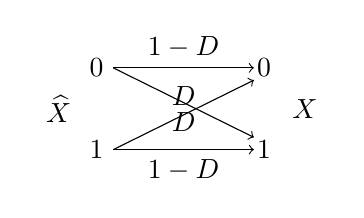
\begin{tikzpicture}[place/.style={inner sep=1pt}]
\matrix
{
    & \node(a1){0};  &    [18mm]     & \node[place](a2){0};        \\
\node{$\widehat{X}$}; &          &              &        &  \node{$\,\, X$};            \\
    & \node(a3){1};  &             & \node[place](a4){1};        \\
};
\draw[->] (a1.east) --node[above]{$1-D$} (a2.west);
\draw[->] (a3.east) --node[above]{$D$} (a2.south west);
\draw[->] (a1.east) --node[below]{$D$} (a4.north west);
\draw[->] (a3.east) --node[below]{$1-D$} (a4.west);
\end{tikzpicture}
\end{center}
\caption{测试信道}\label{fig:F}%BSC
\end{figure}
当 $ D \geq p $ 时, 取 $ \widehat{X} = 0 \Rightarrow \E[d(X,\widehat{X})] = p \leq D $。
综上 : $$ R(D) = \begin{cases} h(p) - h(D) & D < p \\ 0 & D \geq p \end{cases} $$

高斯信源在平方误差失真度量下率失真函数的计算

当 $ D \leq \sigma^2 $ 时,
\begin{align*}
I(X; \widehat{X}) & = h(X) - h(X | \widehat{X} ) \\
	& = { 1 \over 2} \log 2\pi e \sigma^2 -  h(X - \widehat{X} | \widehat{X} ) \\
	& \geq { 1 \over 2} \log 2\pi e \sigma^2 - h(X - \widehat{X}) \\
	& \geq { 1 \over 2} \log 2\pi e \sigma^2 - { 1 \over 2} \log 2 \pi e D  \\
	& = { 1 \over 2} \log \frac{\sigma^2}{D}
\end{align*}
设 $Z = X - \widehat{X}$, 当 $ Z \sim N(0, D)$ 且 $Z$ 与 $\widehat{X}$ 相互独立时不等式成立。

当 $ D \geq \sigma^2 $ 时, 取 $ \widehat{X} = 0 \Rightarrow \E[d(X,\widehat{X})] = \sigma^2 \leq D $。

综上 : $$ R(D) = \begin{cases} {1 \over 2} \log \frac{\sigma^2}{D} & D < \sigma^2 \\ 0 & D \geq \sigma^2 \end{cases} $$

\end{document}







